\documentclass[11pt,a4paper]{article}
\usepackage[utf8]{inputenc}
\usepackage{amsmath}
\usepackage{amsfonts}
\usepackage{amssymb}
\usepackage{graphicx}
\begin{document}
\section{Software process models: waterfall}
\subsection{Koncept}
\subsubsection{Software engenering}
Man begyndte at bruge Software engenering, da der var stor kompleksitet ved projekterne og der skete mange fejl.\\
Man kigger på 
\begin{itemize}
\item Specifikation
\item Design og implementering
\item test og validation
\item Evolution – changing the system in response to changing customer needs
\end{itemize}
Software process model: Abstrakt repræsentation af process

\subsubsection{Waterfall}
Det er en plandriven model, hvilket betyder man starter ud med at ligge hele planen og den følger man så uden at kigge tilbage.\\
Man starter ud med at lave krav, som man så ikke ændre senere, hvor efter man går videre og design fasen, konstruktion, integration, test, installation og så til sidst vedligholdelse.

Man bør bruge den hvis man arbejder med embedded systems, livskritiske systemer eller meget store systemer, da det her kan være svært at lave det samarbejde, som de agile modeller kræver.

Den kræver kun man har kunden indover ved skift mellem phaser.\\
Det er godt hvis ens kontrakt limiter kravene fra starten af.\\
Vi bruger en \textit{Do everything we agreed on} tilgang, da det mindser risikoen for fejl og kunden får alt hvad de har bedt om.\\
Der er meget lidt samarbejde i teamet ud over ved aflevering, da alle opgaver er sat.\\
Prisen er gerne bestemt på forhånd, da man allerede ved hvad der skal ske.
\subsection{pro/con}
Waterfall er rigtigt godt hvis man har en kontrakt der meget specifikt beskriver hvad der er for nogle krav, som man skal igennem.\\
Den fungere ikke hvis man har et projekt hvor der er konstant skiftende krav, da den ikke tillader man går tilbage og ændre i krav.\\
Korte projekter er ofte lette er overskue fra starten af, så der er ikke nogen grund til at bruge den ekstra energi på en agil model.\\
Man sætter sig ud for hvad ens mål er fra starten af, så alle ved hvor det er man vil hen.\\
Der bliver dokumenteret rigtigt godt, da der er mulighed for at det er forskellige teams, som står for de enkelte steps.\\
Man har sjældent kunde/end user med ind over igennem processen, så der er mulighed for at man ender ud med noget andet end det de vil have, da de sjældent ved hvad det er de vil have.
\subsection{Andre emner}
Software process model: incremental and iterative\\
Software process model: integration and configuration\\
Kombinering
\newpage
%-------------------------------------------%
\section{Software process model: incremental and iterative}
\subsection{Koncept}
\subsubsection*{Software engenering}
Man begyndte at bruge Software engenering, da der var stor kompleksitet ved projekterne og der skete mange fejl.\\
Man kigger på 
\begin{itemize}
\item Specifikation
\item Design og implementering
\item test og validation
\item Evolution – changing the system in response to changing customer needs
\end{itemize}
Software process model: Abstrakt repræsentation af process
\subsubsection*{Inkrementiel / Iterativ}
Man kombinere krav, udvikling og validering.\\
Det kan både være plandriven, agilt og oftest et mix.\\
Man udvikler en lille del af produktet (fx UI) får så feedback hvor efter man kan gå videre med den næste del.
\subsection{pro/con}
Man kan bruge både plan-baseret og agil, hvilket giver mulighed for at bruge den model, som man føler sig mest tryk med.\\
Det er let at få feedback.\\
Der er mulighed for at aflevere brugbar software tidligere, da man hele tiden fokusere på enkelte fonktioner.\\
En manager har brug for at få regulær updates, da det er meget svært at overværer processen.\\
Der kommer let noget rodet koden, som increments bliver tilføjet.

\subsection{Andre emner}
Software process model: Waterfall\\
Software process model: integration and configuration\\
Kombinering
\newpage

%-------------------------------------------------
\section{Software process model: integration and configuration}
\subsection{Koncept}
\subsubsection*{Software engenering}
Man begyndte at bruge Software engenering, da der var stor kompleksitet ved projekterne og der skete mange fejl.\\
Man kigger på 
\begin{itemize}
\item Specifikation
\item Design og implementering
\item test og validation
\item Evolution – changing the system in response to changing customer needs
\end{itemize}
Software process model: Abstrakt repræsentation af process

\subsubsection*{Integration and configuration}
Man kigger meget på software, som allerede er blevet udviklet og om man kan genbruge noget af det.\\
Når der bliver kodet noget nyt sørges der for at der er mulighed for at genbruge det ved at configurer det, da det giver mulighed for at sparer tid/penge.
\subsection{pro/con}
Da man genbruger ting bliver der en mindre risiko for at ting ikke virker, men folk får ikke når så meget en ejer følelse af det hvilket kan sænke kvaliteten af det generelle produkt.\\
Der er en risiko for at man bliver nødt til at gå på kompromi med krav hvis man ønsker at bruge allerede udviklet software, som ikke lever helt op til kravene.
\subsection{Andre emner}
Software process model: Waterfall\\
Software process model: incremental and iterative
\newpage
%----------------------------------------------------
\section{Comparison of plan-driven and agile software engineering processes, including analysis of home grounds}
\subsection{Koncept}
Plandriven tror på at et resultat kan blive forudset, hvor et agilt forventer at der kommer ændringer og tager højde for dette for at det skal give den bedste value.\\
\textbf{CI} clean build af systemet flere gange om dagen. I det agile builder man mange gange for at se om det virker.\\
\textbf{Prototype} lave krav sammen med kunde. Prototype ved agile kan vises som et færdigt produkt efter hver iritation og så udvikle på den så det kan ses hvilken retning kunden vil.\\
\textbf{XP practices} Pair programming, planning game, TDD\\
\textbf{Scrum roles} Product Owner, ScrumMaster, Development Team\\
\textbf{Practices} collaborative, Open communication, adaptation, trust, Sprint Planning+Daily Scrum+Sprint Review+Sprint Retrospective,+Baclog refinement.\\
\textbf{Home ground}\\
\begin{tabular}{|c|c|}
\hline 
\textbf{Plan-driven} & \textbf{Agile} \\ 
\hline 
Plan orientede udviklere (mix af skill) & Velvidende, samlet og samarbejede udviklere \\ 
\hline 
Mix af kunde kababilitet nuveauer & højt empowered kunder \\ 
\hline 
God dokumentation & Forventer ofte ændringer \\ 
\hline 
Krav kendt tidligt og forsøgt at set kommende & Ændringer er billige \\ 
\hline 
At lave om er dyrt & Mindre teams \\ 
\hline 
Store teams & Hurtig ”value” \\ 
\hline 
Høj sikring & • \\ 
\hline 
\end{tabular} 


\subsection{pro/con}
Agile er til små\\
Plan-driven er til store\\
Mix
\subsection{Andre emner}
Software process model: Waterfall\\
Software process model: incremental and iterative\\
integration and configuration

\newpage
%----------------------------------------------------
\section{Key features of Scrum}
\subsection{Koncept}
A framework within which people can address complex adaptive problems, while productively and creatively delivering products of the highest possible value.
\begin{itemize}
\item Roles\\ \textbf{Product Owner}: Ejeren af produktet, derfor ikke en del af teamet, men hjælper med at sætte krav.\\ \textbf{Scrum Master}: Styrer teamet i forhold til hvad der skal ske hvornår, er ikke en del af teamet.\\ \textbf{Team}: Programører, designere mm.
\item \textbf{Sprint Planning}: Planlægning.
\item \textbf{Daily Scrum}: Dagligt møde.
\item \textbf{Sprint Review}: Review afholdt ved afslutningen af hvert sprint.
\item \textbf{Sprint Retrospective}: Møde omkring hvad gik godt, hvad kan gøres bedre og hvad vil vi gøre for at gøre det bedre.
\item \textbf{Backlog refinement}: Holde backlog opdateret.
\item \textbf{Product Burndown/Sprint Burndown}: Completed work per day for det nuværende projekt udgivelse.
\item \textbf{Scrum board}: Fremvisning af backlog
\end{itemize}
Scrum giver \textbf{commitment}, \textbf{courage}, \textbf{focus}, \textbf{openhed} (team) \textbf{respect} (management over for team, derfor tror de på de gør deres arbejde)

Det sker nogen gange følgende \textbf{fejl}: Scrum master implemented as manager who tells team what to do (right way: Facilitator for team), kunde bliver ikke involveret, nye krav og opgaver bliver tilføjet i løbet af et sprint.

\textbf{eXtreame Programing} er godt ved scrum i forhold til kunde-on-site, user stories, planning game.
\subsection{pro/con}
Effektivt brug af tid og penge\\
Gøre store projekter mere overskulige\\
Godt for hurtigt bevægende projektor\\
Teams for godt overskulighed\\
Adopts feedback\\
Man kan se arbejdet hver person laver\\
Ens scope kan let blive uroligt\\
Hvis folk ikke er committet går det let galt\\
Kan være svært at få igang i store teams\\
Daglige møder iritere folk\\
\subsection{Andre emner}
Agile
\newpage
\section{Key features of RUP}
\subsection{Koncept}
Framework til UP, altså et RUP produkt.\\
Interativ process framework.\\

Udviklet i små tidsboksede iterationer.\\
High-value og high-risk tidligt. Forsøg med genbrug.\\
Dette forsikre kunder om value.\\
Være klar på ændringer tidligt i processen.\\
Team work er vigtigt.\\
4 phaser: Inception, elaboration, construction, transition.

\begin{figure}[h!]
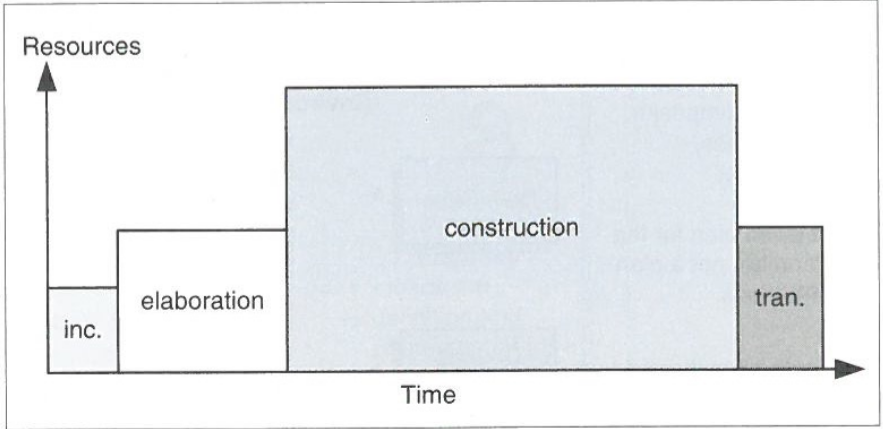
\includegraphics[scale=1]{rup.png}
\end{figure}
\underline{Inception}: Establish, project schedule and cost estimate, gennemførlig\\
Make mussiness case, define scope.
 
\underline{Elaboration}: Address know risk factors, establish and validate system architecture, mange system requirements, plan for the construction phase (cost og schedule)
 
\underline{Construction}: Lave det sidste, series of short time-boxed iterations, usecase, UML

\underline{Transition}: deploy, feedback for refinements, user training\\
\textbf{Discipline}

Requriment, design, test, implemtering, projekt mangement\\
\textbf{Best practice}

Timeboxed iterations, reuse, vertify quality, visual modelling, manage requirements, manage change.\\
\textbf{Misforståelser}

Iteration bliver for lang\\
De bliver ikke time boxed (bliver udvidet)\\
De ender ikke i test/integret\\
\textbf{Scum}: If the predefined optional activities of UP is seen as requried tasks it is bad, but if they are seen as optional advice it is okay.\\
\textbf{XP}:Upfront moddeling: UP uses accepts much more time\\
Early iteration: XP does not look for high-value and high-risk but might find them\\
\subsection{pro/con}
Pros: RUP takes the best parts of Waterfall and incorporates them into a more iterative process that allows for changes.\\
Cons: Like Waterfall, RUP is also process-heavy, and can rely too heavily on stakeholder feedback. Even as an iterative process it can be too slow for certain types of projects.
\subsection{Andre emner}
Scrum
\newpage
\section{Requirements Elicitation and Management}
\subsection{Koncept}
\textbf{Main activites} finde og analysere needs, specificere krav, validere krav.\\
\textbf{Organized} spiral: requirement validation, risk analysis, models and prototype.\\
\textbf{Requirements elicitation}: find og forstå krav, organiser dem, prioter, dokumenter, forfra.\\
\textbf{Techniques} interview (open/closed), etnography (observer), prototype.\\
\textbf{communicate}: Stories/senaries\\
\textbf{Dokument}

Waterfall: Approved requirements document with strict change management

Scrum: Product vision and product backlog, reviewed and updated every sprint\\
\textbf{negotiated}

Waterfall: Up front in the requirements phase – state it now or it will be difficult later to get it

Scrum: Ongoing refinement of product backlog with stakeholders, say what is most important now, we will continue
\subsection{pro/con}
Mange kunder har krav som modgår hinanden, de snakker deres egent sprog så der sker let forvirring.
\subsection{Andre emner}
Configuration Management
\newpage
\section{Managing change to requirements}
\subsection{Koncept}
De bliver manged for at man kan holde styr på de krav som kommer fra kunderne, så man kan se om man får klaret dem.\\
Man kigger også efter de versioner man laver af software, så det er muligt at gå tilbage og se hvad der er sket.\\
Ændringer bliver godkendt af forskellige personer alt efter modellen der bliver brugt. I en plan driven er det ofte en projekt manager eller en styregruppe og ved en agil er det kunden.\\
Får at holde prisen nede kan man arbejde ud fra expect changes hvor man fx laver prototyper, så kunden let kan se hvad der sker eller tolerance to changes hvor man designer så det er let at lave ændringer.\\
$Exposure(r)= P(r) * L(r)$
\subsection{pro/con}
\textbf{Prototype} den bliver brugt anderledes end hvordan det endelige produkt skal bruges. Den bliver ikke brugt af de "endelige" brugere. Der bliver ikke brugt nok tid på at træne brugerne i at bruge den.\\
\textbf{incremential development}\\
Kunder kan bruge det som prototyper som bliver vidre udviklet. De kan se værdig tidligt. Let at få ændringer ind undervejs.\\
Problematisk hvis det er hele systemer der skal laves ændringer i eller hvis det skal arbejde sammen med gamle systemer. Svært at definere en del base for hele systemet tidligt i udviklingen. 
\subsection{Andre emner}
Configuration Management
\newpage
\section{Quality Control: Verification and Validation}
\subsection{Koncept}
\textbf{Validation}: Are we building the right product?\\
\textbf{Verification}: Are we building the product right?\\
\textbf{Inspection}: Analyser, check system krav, design modeller, soruce code, test.\\
\textbf{Test}: living up to the requriments, code folows the design, models, requriments\\
\textbf{Peer review}: peers to check your code and more\\
\textbf{TDD}: Vi skriver en test og ud fra den udvikler det. Dette gør at vi ved det virker før vi går vidre og det tvinger os til at skrive tests hvilket ellers godt kan være noget som man kommer til at hoppe over.\\
\textbf{regressiontest} re-running previous tests\\
\textbf{agile practices} Definition of Done, Sprint Review, Check before check-in, Never break the build, Fix problems when you see them, Culture, XP: Customer on site, XP: Pair programming
\subsection{pro/con}
It can help to prevent faulty goods and servies being sold\\
It does not prevent waste of resources when products are faulty
\subsection{Andre emner}
Quality Management
\newpage
\section{Risk Management}
\subsection{Koncept}
Something that may happen and causes a loss\\
\textbf{Kategorier} Catastrophic, Critical, Marginal, Negligible, Uncertainty, project, technical, business\\
- Keyperson from team dies, a supplier is not delivering as promissed

\begin{figure}[h!]
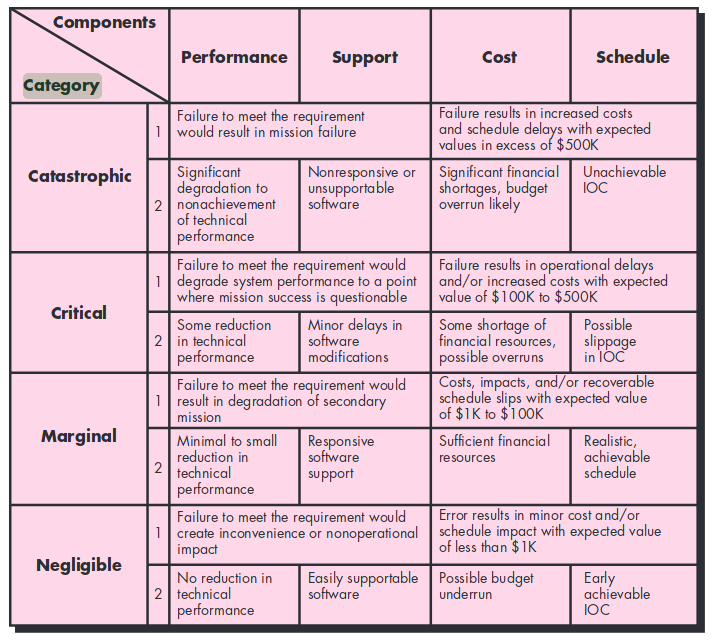
\includegraphics[scale=1]{risk-cat.png}
\end{figure}
\textbf{how} 
\begin{itemize}
\item Identifiser, udregn exposure, beskriv
\item Priotiser
\item RMMM
\end{itemize}
\textbf{Waterfall / plan driven} en del af planerne, del af andre planer, det bliver planlagt hvordan.\\
\textbf{agile} Daily Scrum, sprint review, sprint retrospective.\\
\textbf{spiral} risk driven, starter hver iteration ud med risk, og gør det tidligt
\subsection{pro/con}
\subsection{Andre emner}
\newpage
\section{Project Planning and Management}
\subsection{Koncept}
\textbf{plandriven project planning} plan arbejdet, gør det, antag du kan forudse hvad der er leveret\\
\textbf{Progress} Milepæle og dokumentation\\
\textbf{Agil planning} Ændringer, prioritiseret backlog\\
\textbf{Estimation} Taget ud fra forud viden, algorime baseret (modeller og parameter)\\
\textbf{Agile estimation} Velocity af story points\\
\textbf{sprint planning} planlægning sammen med scrummaster, productowner og teamet\\
\textbf{Planning game i XP} For hver opgave giver man et estimat på hvor lang tid det ca tager. Kortest vs længest diskuterer hvorfor de synes det.
\subsection{pro/con}
\subsection{Andre emner}
\newpage
\section{Quality Management: How is quality defined - agile versus plan driven approaches}
\subsection{Koncept}
Forskellen mellem plandreven og agilt er at plandreven går ud fra at man kan forudsige resultatet, og agilt forventer at ændringer kommer til at ske.\\
Hvordan definerer Böhm / Turner de \textbf{primære faktorer}?
\begin{itemize}
\item Applikation er små, hurtige ændringer, turbulent environment
\item Management onsite, kvalitetskontrol, stilletiende viden
\item Teknisk: Prioriterer uformelle requirements og simplet design
\item Mennesker: Cockburn L2 og L3 udviklere
\end{itemize}
Grunden til at requirements ændrer sig kan være forretningsmæssige, teknologiske eller fordi de lærer at bruge det.\\
Hvis at noget skal ændres, så kan man ændre process og analysere impakten på ændringen

\begin{figure}[h!]
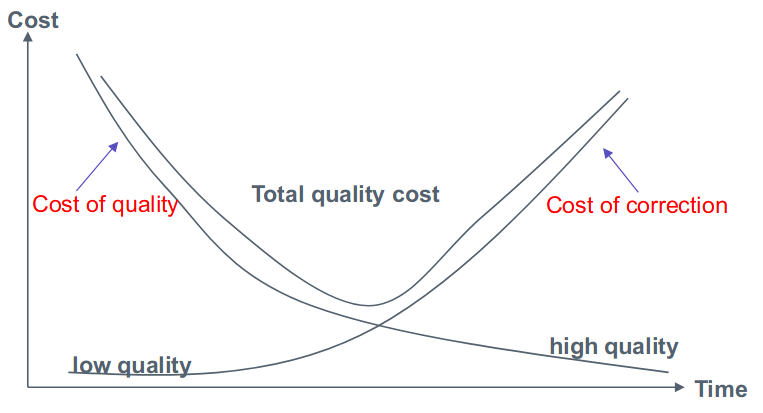
\includegraphics[scale=1]{quality-mang.png}
\end{figure}

Trade of er at man vælger noget fram for noget andet fx man tester mindre for at blive hurtigere færdig.\\
\textbf{Quality culture} alle føler sig ansvarlige for softwaret\\
\textbf{Agile} Meget relesable code, unscheduled product reviews, schilude reviews, status møder, mange tests.\\
\textbf{Pair programming} to programører skriver sammen, man kan skrive tests samme tidigt med koden skrives, fejl findes tidligt, det er god kode deling til hvis en fx stopper.\\
\textbf{Validation}: Are we building the right product?\\
\textbf{Verification}: Are we building the product right?\\\\

\subsection{pro/con}
Quality Management assumes good process  good --> product, or same process delivers same quality
\subsection{Andre emner}
\newpage
\section{Configuration Management}
\subsection{Koncept}
Disciplin som giver en måde til at identificere og controllere ting. Det giver en måde at håndtere integritet og kvalitet.\\
Branching fordele opgaver ud i forskellige grene, så man ikke arbejder i de samme filer.\\
Merging sætte ændringer sammen fx fra grene.\\
\textbf{VC system}\\
Centralize: En fælles kopi som alle sender til\\
Distributed: Alle har meta data, kan gøre det samme som centralized. Hvis man har mange ændringer eller mange binærer filer kan det komme til at fylde rigtigt meget\\
\textbf{Release}: ALT!\\
\textbf{Continous integration}: Agile teams typically configure CI to include automated compilation, unit test execution, and source control integration. Sometimes CI also includes automatically running automated acceptance tests.\\
\textbf{Daily build}: Performing daily builds helps ensure that developers can work knowing with reasonable certainty that any new bugs that show up are a result of their own work done within the last day.
\subsection{pro/con}
\textbf{Plandriven}\\
Strong emphasis on testing\\
Validation of internal and external deliverables not just the product.\\
Definition of requirements before designing the system.\\
Enable project management to track the progress very accurately. The completion of each phase is a milestone in the project plan.\\
Does not handle concurrent events.\\
Does not handle iterations.\\
Can't handle the dynamic changing of requirements during the lifecycle.\\
\textbf{Agile}\\
Not optimized for sprint
Slow for testing\\
easy share\\
easy release

\subsection{Andre emner}
\newpage
\section{Andet}
\subsection{Scrum}
\textbf{Roles}\\
\textit{Product Owner:} Ejeren af produktet, derfor ikke en del af teamet, men hjælper med at sætte krav.\\
\textit{Scrum Master}: Styrer teamet i forhold til hvad der skal ske hvornår,
er ikke en del af teamet.\\
\textit{Team}: Programører, designere mm.\\
\textbf{Sprint Planning}: Planlægning.\\
\textbf{Daily Scrum}: Dagligt møde.\\
\textbf{Sprint Review}: Review afholdt ved afslutningen af hvert sprint.\\
\textbf{Sprint Retrospective}: Møde omkring hvad gik godt, hvad kan gøres
bedre og hvad vil vi gøre for at gøre det bedre.\\
\textbf{Backlog refinement}: Holde backlog opdateret.\\
\textbf{Product Burndown/Sprint Burndown}: Completed work per day for det nuværende projekt udgivelse.\\
\textbf{Scrum board}: Fremvisning af backlog\\
Scrum giver commitment, courage, focus, openhed (team) respect
(management over for team, derfor tror de på de gør deres arbejde)
\subsection{Continuous integration (CI)}
Samling af alt minimum 1 gang om dagen i XP mange gange om dagen.
\subsection{Prototype}
Prototype lave krav sammen med kunde. Prototype ved agile kan vises som et færdigt produkt efter hver iritation og så udvikle på den så det kan ses hvilken retning kunden vil.\\
Får at holde prisen nede kan man arbejde ud fra expect changes hvor man fx laver prototyper, så kunden let kan se hvad der sker eller tolerance to changes hvor man designer så det er let at lave ændringer.
\subsection{Home ground}
\begin{tabular}{|l|l|}
\hline 
• & Agile  \\ 
\hline 
Prmær mål & Hurtig værdi, god til ændring  \\ 
\hline 
Størelse & Mindre teams og projektere  \\ 
\hline 
Envioment & Turbulent, høj chance, projekt dokuseret  \\ 
\hline 
Kunde relation & On-site kunder, fokus på increments  \\ 
\hline 
Plan/kontrol & Kvalitet over kvuantitet  \\ 
\hline 
Kommunikation & Interpersonal knowledge  \\ 
\hline 
Krav & priotiserede informative historier og test cases, kan klarer uforusete ændringer  \\ 
\hline 
Udvikling & Simpelt design, små increments, refactor billigt  \\ 
\hline 
Test & udførbarer test cases definere krav  \\ 
\hline 
Kunde & Dedicted  \\ 
\hline 
Udviklere & ingen under level 2 cockburn  \\ 
\hline 
\end{tabular} 
\begin{tabular}{|l|l|}
\hline 
• & Plan-driven \\ 
\hline 
Prmær mål  & Forventning, stabil, høj sikkerhed \\ 
\hline 
Størelse  & Støre teams og projektere \\ 
\hline 
Envioment & Stabilt, lav ændring, projekt/organzition fokus \\ 
\hline 
Kunde relation & As-needed customer, kontrakt, evolutionary \\ 
\hline 
Plan/kontrol Kvuantitet og kvalitet \\ 
\hline 
Kommunikation & Dokumenteret knowledge \\ 
\hline 
Krav & Formaliseret projekt, interface qualitet, forudser krav \\ 
\hline 
Udvikling & Akitecht paralel udvikling, længre incrementer, refactor er dyr \\ 
\hline 
Test & Dokumenteret test planer og procedyrer \\ 
\hline 
Kunde & ikke altid sammen \\ 
\hline 
Udviklere & Level 3 tidigt efter følgende få; 30 1B \\ 
\hline 
\end{tabular} 
\subsection{Requirement/ændringer}
Krav er stillet af kunden til noget produktet skal kunne når det er færdig udviklet\\
Ved plan-driven stilles de alle sammen til at starte med.\\
Ved agile de stilles under vejs, da der tages højde for der kan komme ændringer.
\subsection{Cockburn}
Level 3: Ændre en metode (Bryde regler) til at passe til en ny ukendt situation.\\
Level 2: Små ændringer for at passe til en kendt ny situation\\
Level 1A: Kan lave metode step med mere advancerede modeller\\
Level 1B: Kan lave metode step med simple modeller\\
Level -1: Kan have tekniske skills, men kan ikke eller vil ikke samarbejde eller bruge en metode.
\subsection{Dokumentation}
Plan-driven kræver god dokumentation, da der let kan ske udskiftning imellem de forskelige faser fx mellem design og udvikling.
\subsection{Negotiated}
Waterfall: Up front in the requirements phase – state it now or it will be difficult later to get it.\\
Scrum: Ongoing refinement of product backlog with stakeholders, say what is most important now, we will continue.
\subsection{Validation}
Are we building the right product?
\subsection{Verification}
Are we building the product right?
\subsection{Inspection}
Analyser, check system krav, design modeller, soruce code, test.
\subsection{Test}
unit, auto, manuel\\
living up to the requriments, code folows the design, models, requri-
ments\\
regressiontest re-running previous tests\\
Pair programming
\subsection{Test Driven Development (TDD)}
Test skrives inden koden skrives som der skal udviles ny funktion. Man går ikke videre indtil det virker.\\
Code coverage. Regression testing. Simpel debug. System dokumentation.
\subsection{Risk Mitigation, Monitoring, and Management Plan (RMMM)}
A risk management strategy can be included in the software project plan, or the risk management steps can be organized into a separate
risk mitigation, monitoring, and management plan. The RMMM plan documents all work performed as part of risk analysis and is used by the project manager as part of the overall project plan.
\subsection{risk information sheet (RIS)}
Dokumentet som informere om den enkelte risk. 
Ofte brugt database system til at kunne lave ændringer.
\subsection{Dimensions}
Personal\\
Dynamism: Krav ændringer / måned\\
Kultur: chaos vs order\\
Antal folk\\
Criticality: Tab i forhold til fejl.
\end{document}
